\Chapter{Frontend Dokumentáció}

A fejezet a felhasználói felületet mutatja be.

\Section{Applikáció létrehozása}
Az Angular applikációt az Angular CLI-vel tudjuk létrehozni. Az
\begin{java}
ng new "projectname"
\end{java} 
parancs használatával jön létre a projektünk. Projekt létrejötte után az
\begin{java}
ng generate component "componentnev"
\end{java}
 használatával tudunk új komponenseket létrehozni.
Az \ref{fig:mappaszerkezet}. ábra egy elkészített program mappaszerkezetét mutatja be.

\begin{figure}[h]
\centering
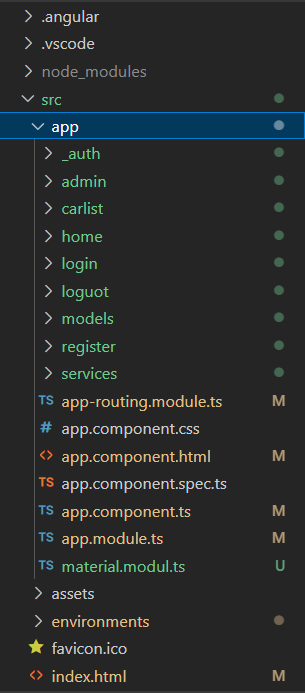
\includegraphics[scale=0.6]{images/angular_mappaszerkezet.png}
\caption{Angular mappaszerkezet}
\label{fig:mappaszerkezet}
\end{figure}
\newpage

\Section{Felhasználói felület}

\subsection{Regisztráció és bejelentkezés}
Itt fog történni a regisztráció. Ez a legelső lépés, hogy tudjuk használni a webalkamazást.
A regisztráláshoz szükséges egy felhasználónév és jelszó kombináció (\ref{fig:regisztracio}. ábra).

\begin{figure}[h]
\centering
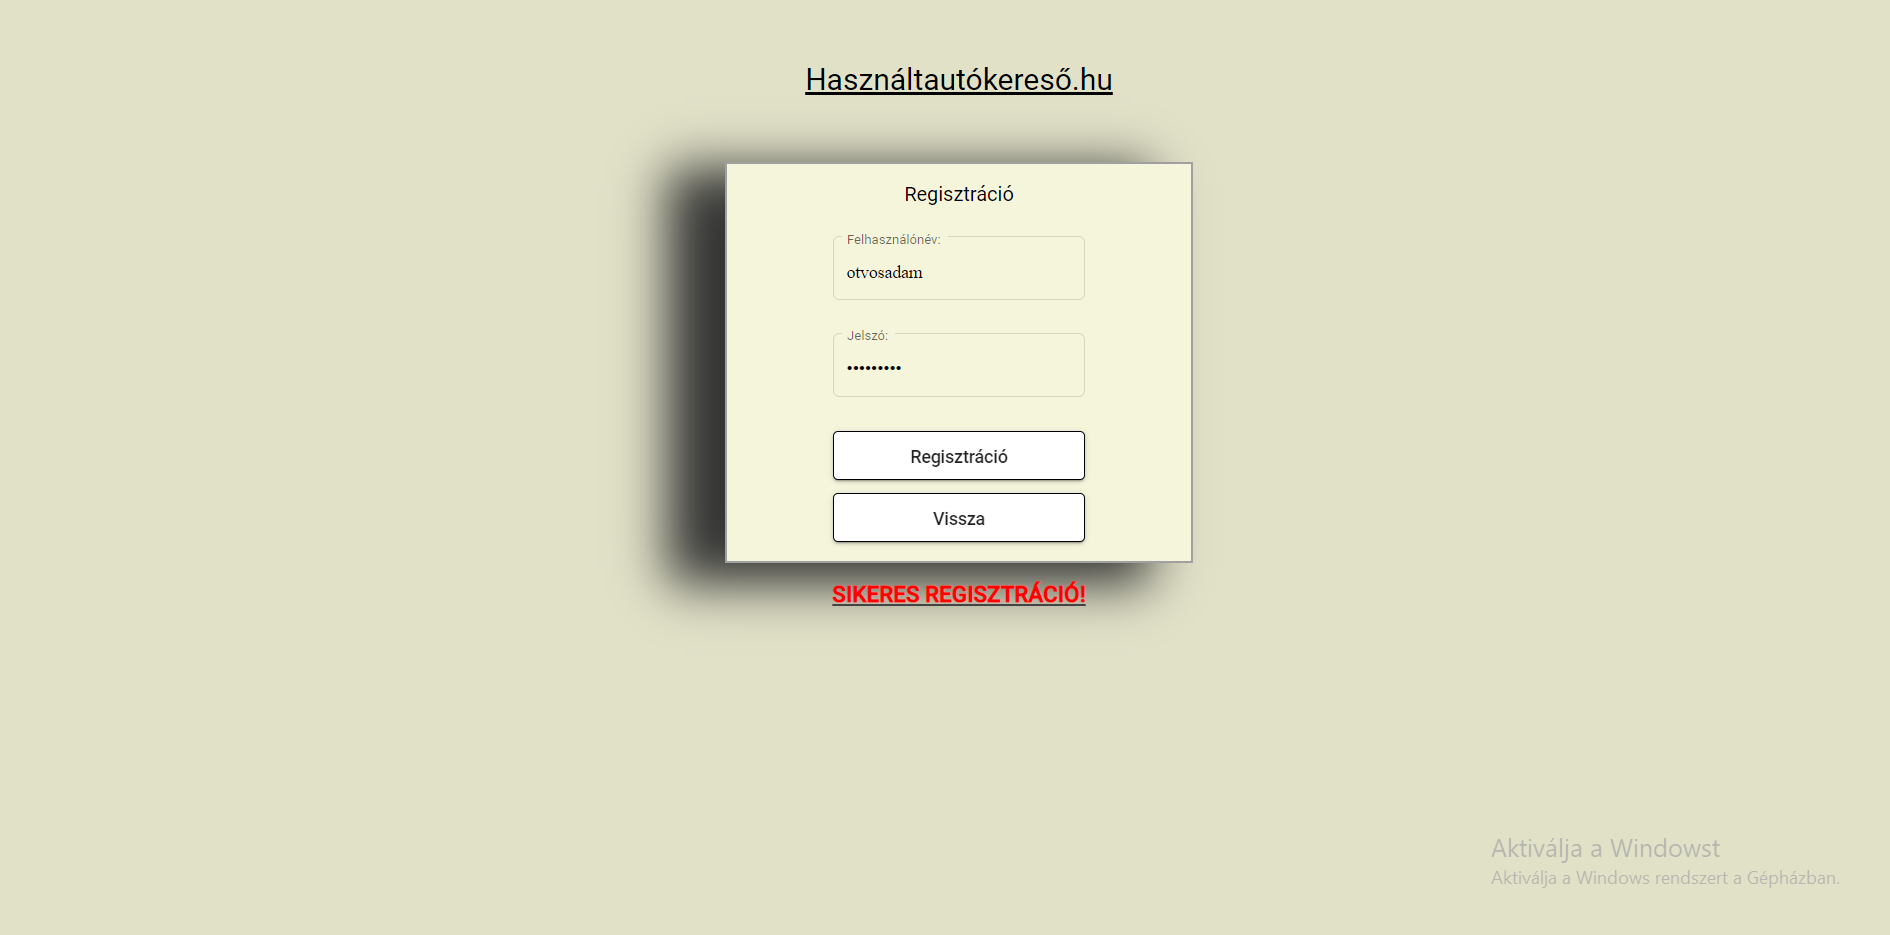
\includegraphics[scale=0.37]{images/regisztracio.png}
\caption{Regisztráció}
\label{fig:regisztracio}
\end{figure}

A felhasználó adatai JSON formátumba lesz elküldve a szerver felé.

Tájékoztatást kapunk akkor is, hogy ha sikerült regisztráció, és arról is ha olyan felhasználónévvel szeretnénk regisztrálni, ami már használatban van, vagy éppen arról ha a jelszó mezőt kitöltetlenül hagytuk.

Miután sikeresen regisztráltunk, vissza is léphetünk a bejelentkező felületre.
A bejelentkező felületen ugyan azzal a felhasználónév és jelszó kombinációval be is tudunk jelentkezni (\ref{fig:bejelentkezes}. ábra).

\begin{figure}[h]
\centering
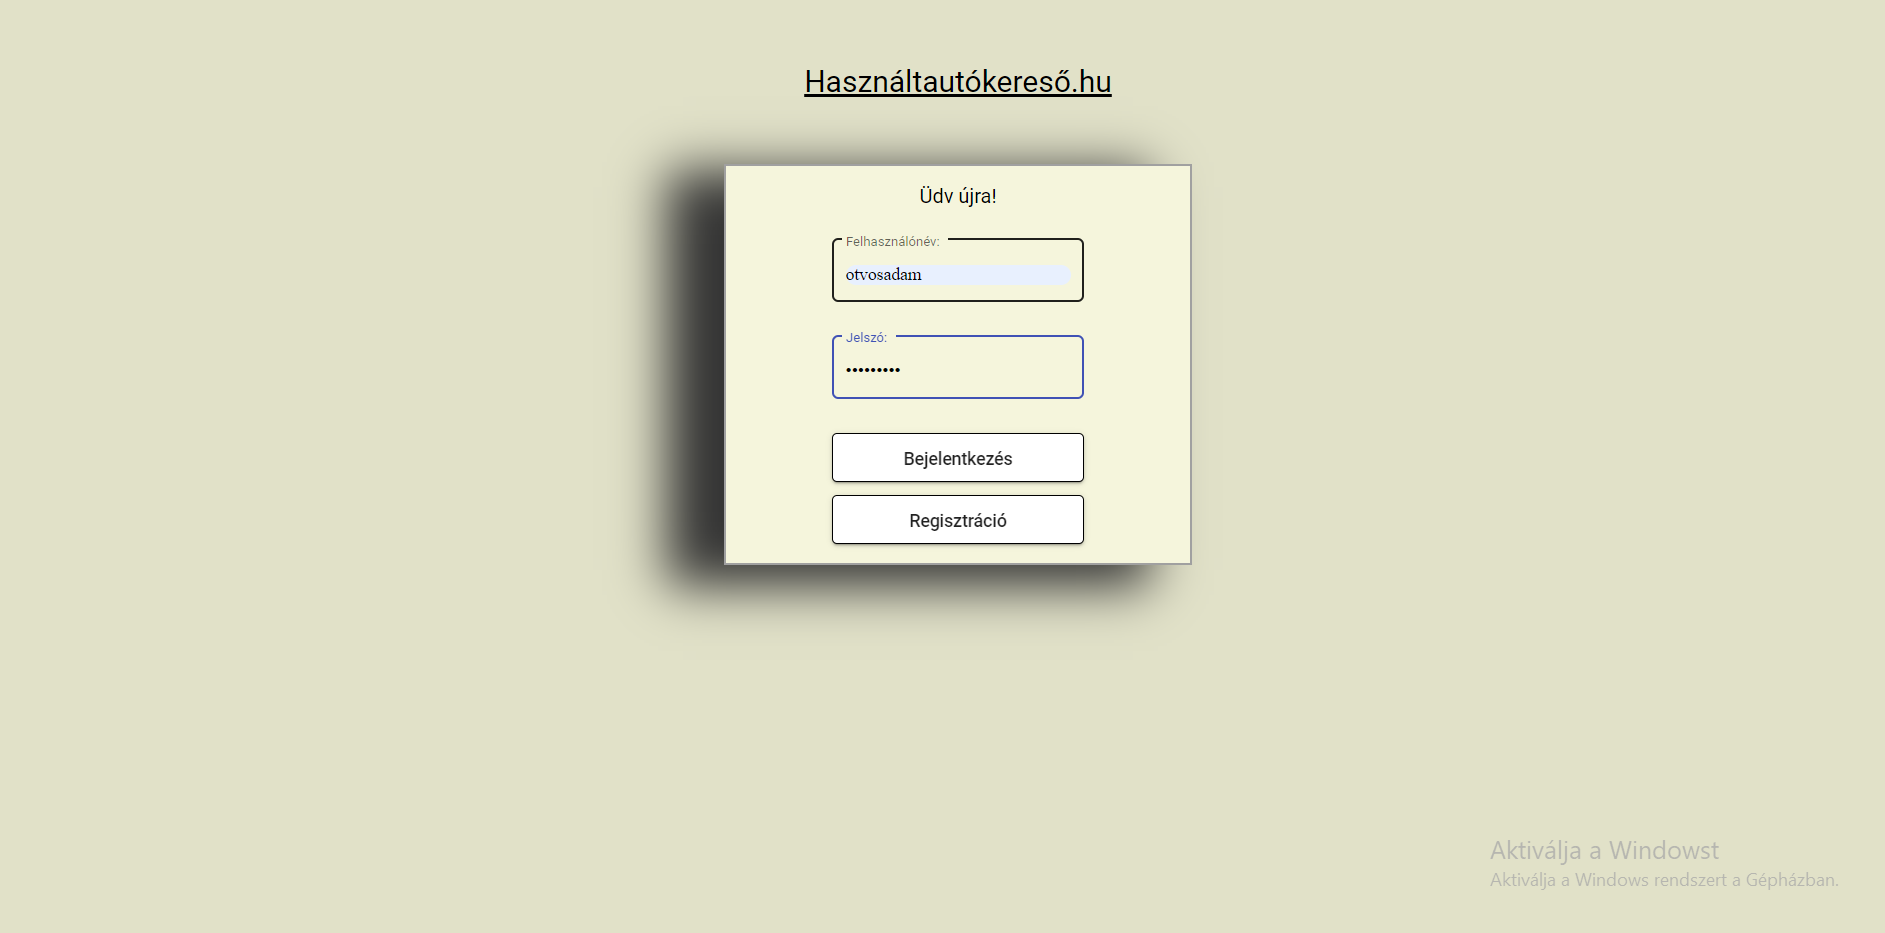
\includegraphics[scale=0.37]{images/bejelentkezes.png}
\caption{Bejelentkezés}
\label{fig:bejelentkezes}
\end{figure}

Ha hibás felhasználónevet vagy jelszót adunk meg, vagy éppen kitöltetlenül hagyunk egy mezőt, akkor tájékoztatást fogunk róla kapni.
Ha nem rendelkezünk fiókkal, a "Regisztráció" gombra kattintva át is jutunk a regisztrációs felületre.

Bejelentkezésnél is JSON formátumban lesznek elküldve az adatok.

Ha sikeresen bejelentkeztünk, akkor kliens kap egy tokent, és egy jogosultságot is amit a Local Storage-ban fog eltárolni addig, ameddig ki nem jelentkezünk az oldalról.

Az alábbi programrész bemutatja, hogyan menthető el a Local Storage-ban az adat.

\begin{java}
public setToken(jwtToket: string) {
    localStorage.setItem("jwtToken", jwtToket);
}
\end{java}
A következő pedig azt mutatja be, hogy hogyan lehet kitörölni az adatokat belőle.

\begin{java}
public logOut() {
    localStorage.clear();
}
\end{java}

Bejelentkezés után átkerülünk a Főoldalra.

\subsection{Főoldal}

A Főoldalon össze tudjuk állítani a keresési feltételeinket ha szeretnénk szűrni az autókat.
A "Keresés" gombra kattintva a kliens lekéri a megfelelő adatokkal rendelkező autókat, eltárolja a Local Storage-ba, és átvezényel minket a találati oldalra.

Ennél a kérésnél az adatokat Query paraméterekben küldi el a szerver felé.

Statisztikákat is tudunk megnézni az Autómárkák keresési számaival kapcsolatban akár dátum függvényében is, és így megtudhatjuk azt például, hogy egy adott évszakban melyik márkára kerestek rá a legtöbben (\ref{fig:Találatok}. ábra).

\begin{figure}[h]
\centering
\includegraphics[scale=0.37]{images/Főoldal.png}
\caption{Főoldal}
\label{fig:Főoldal}
\end{figure}

A maximális dátum amit ki lehet választani, az mindig automatikusan változik annak függvényében, hogy éppen hanyadika van.
A kezdő dátum sosem lehet nagyobb a végső dátumnál, és a végső dátum sem lehet kisebb a kezdő dátumnál, ezt a rendszer automatikusan nem engedi.

A diagramot a Chart.js \cite{Chartjs} segítségével készítettem el. 
\begin{java}
npm i chart.js@2.9.4
\end{java}
paranccsal adtam hozzá az Angular projektemhez.

A Chart.js \cite{Chartjs2} egy diagram rajzoló, ingyenes JavaScript-könyvtár HTML-alapú diagramok létrehozására. Ez az egyik legegyszerűbb JavaScript vizualizációs könyvtár, ami több diagram típust is támogat például:

\begin{itemize}
\item vonaldiagram,
\item oszlopdiagram,
\item kördiagram,
\item buborékdiagram.
\end{itemize}

A következő kódrész bemutat egy példát oszlopdiagram létrehozására.
\begin{java}
new Chart(this.ctx, {
      type: "bar",
      data: {
         datasets: [{
           label: "Keresesi statisztika",
           data:this.
           dataSearch,
           backgroundColor: "rgb(115 185 243 / 65%)",
           borderColor: "#007ee7",
           fill: true,      
          },
         ],
         labels: this.data
       },
       options: {
         events: ['none'],
         scales: {
            yAxes: [{
             ticks: {
              beginAtZero: true
          }
       }]
     }
   }
}); 
\end{java}

Külön be lehet állítani rajta, hogy az oszlopok milyen színűek legyenek, hogy honnan kezdődjön a diagram y oszlopának számozása, adhatunk hozzá jelmagyarázatot. A Chart.js segítségével teljesen testreszabhatjuk a diagramunkat.

Ahogy már az előző fejezetben is említettem, a csavarkulcsot csak az Admin fel-
használó látja, és így csakis ő tudja használni. Amikor rá kattint átkerül az Admin felületre.

Ha nem vagyunk Admin felhasználók, akkor ha megadjuk az elérési útvonalát akkor automatikusan a bejelentkező felületre kerülünk, hogy tudjuk magunkat igazolni.

Az Angular AuthGuard \cite{Authguard} bővítményével valósítottam meg az útvonal védelmet, amit a parancssorban a 
\begin{java}
ng g guard auth
\end{java}
parancsal hoztam létre.
Az AuthGuard biztosít egy \textit{canActivate} eseményt, ami az útvonal elérése előtt hívódik meg, és ha rendelkezünk a megfelelő jogosultsággal, akkor beenged minket az adott lapra, viszont ha nincs hozzá jogunk, akkor megtudjuk azt is adni, hogy hova irányítson át minket a weboldalon belül.

\subsection{Találatok}

Itt tudunk böngészni az autók között, és amikor kiválasztjuk a magunknak megfelelő autót akkor a megtekintés gombra kattintva eljutunk arra a weboldalra, ahol hirdetik az autót, és ott bővebb információt is találhatunk róla (\ref{fig:Találatok}. ábra).

\begin{figure}[h]
\centering
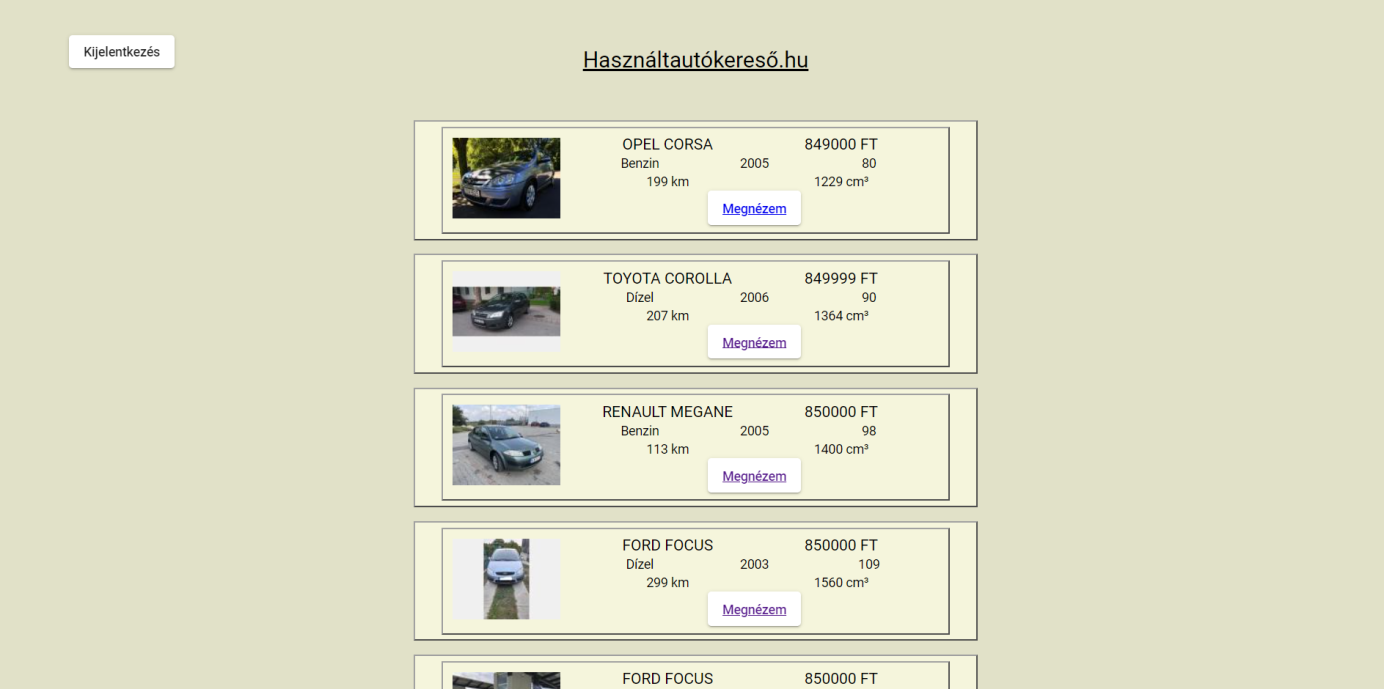
\includegraphics[scale=0.9]{images/Talalatok_FE.png}
\caption{Találatok}
\label{fig:Találatok}
\end{figure}

Az oldalon az autók a Local Storage-ból töltődnek be, tehát ha újra töltjük az oldalt akkor sem fog eltűnni a keresésünk, hanem az utolsó keresési előzményünk lesz benne. Ha kijelentkezünk akkor ezek az adatok is törlődni fognak a Local Storage-ból.
\newpage

\subsection{Adminisztrátori felület}

Az adminisztrátori felületet csak az Admin jogosultsággal rendelkező felhasználó tudja elérni, és itt tudja az Adminisztrációs feladatokat elvégezni (\ref{fig:Admin}. ábra).

\begin{figure}[h]
\centering
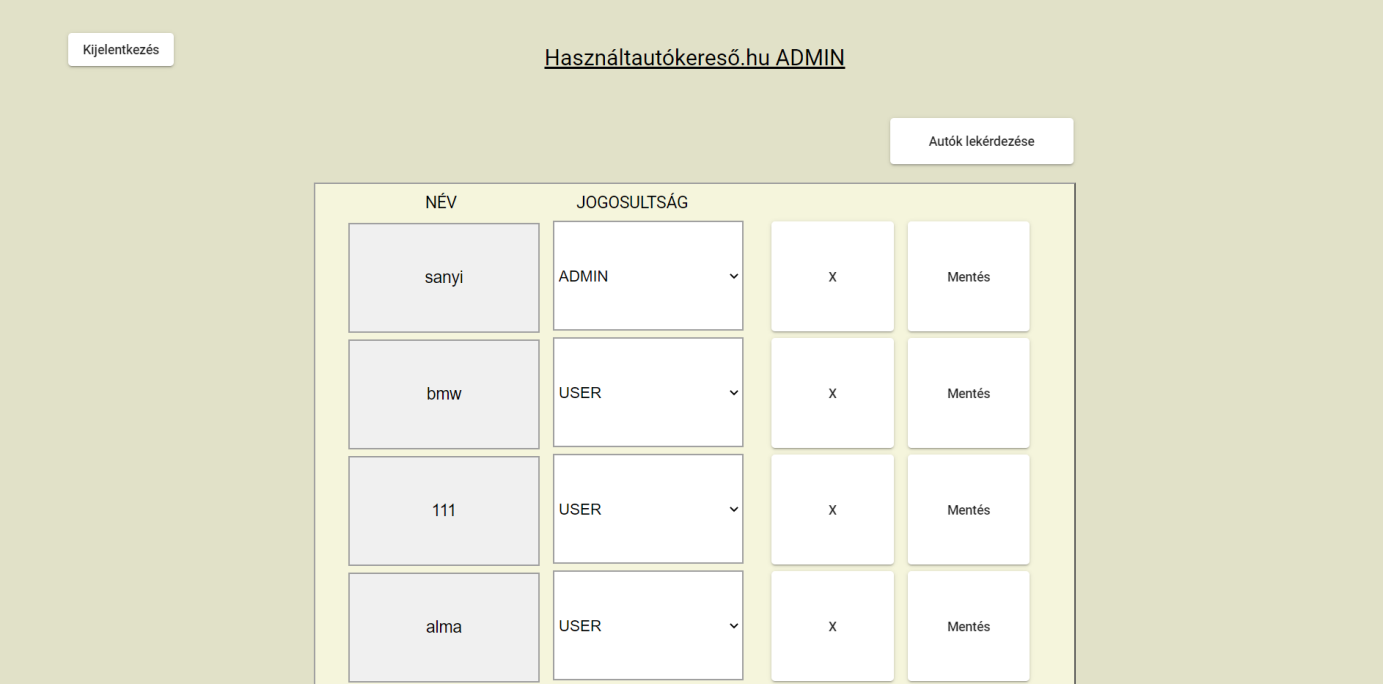
\includegraphics[scale=0.9]{images/Admin_FE.png}
\caption{Admin Felület}
\label{fig:Admin}
\end{figure}

Van egy "Autók lekérdezése" gombunk, amit ha megnyomunk,  akkor egy kérést indítunk el a szerver számára, hogy frissíteni szeretnénk az autókat. Ez a lekérdezés kettő oldalról gyűjt össze autókat az egyik a Használtautó.hu, a másik pedig a JóAutók.hu.

Az Adminnak lehetősége van a felhasználók jogosultságának megváltoztatására, ami lehet Admin vagy User. Utána a mentés gombbal el is tudja azt menteni.

Lehetőség van a felhasználó kitiltására vagy törlésére a "törlés" gombra kattintva, és utána már azzal a felhasználói fiókkal már nem lehet bejelentkezni.


